\chapter{Results}
\label{chap:results}

As stated in Chapter~\ref{chap:methodology}, due to the absence of an events
dataset, it is not possible to extensively study the system's accuracy.
However, this chapter presents illustrative examples when the proposed pipeline
was applied to real data.

It was considered 7 months of measurements, from may to November 2016.
This data was then split in batches of 10 days, and for each batch,
a complete offline analysis was executed.
Considering the 35 servers, the mean number of client-server
pairs, in which occurred at least one measurement between them during a batch,
was 2246.
After the End-Users Filtering step, this average reduced to 741.
In general, one client measured against a single server through the batch.

For all cases, the time series were preprocessed with a median filter.
The change points were detected through the optimization model described in
Chapter~\ref{chap:change_point_detection}.
For each QoS metric, the algorithms' hyperparameters were manually selected.
It was opted by conservative values, in order to avoid change points that,
through a visual inspection, may be arguably not related to a network event.
These algorithms choices were guided by two facts.
First, through a empirical visual analysis,
it was verified their reasonable performance with real data.
Also, the impact of their hyperparameters can be easily interpreted, which is
an important feature for manual tuning.

The fraction of clients threshold, used to check if an event can be
located in a vertex, was set to 0.75. The $\delta$ parameter, used to verify if
two change points are near, was set to 8 hours.

Section~\ref{sec:possible_correct_outcomes} presents examples with potential
correct outcomes, and Section~\ref{sec:possible_wrong_outcomes} exposes
cases with possible wrong results. These conclusions were manually corroborated
with a visual check.

\section{Possible Correct Outcomes}
\label{sec:possible_correct_outcomes}

Figure~\ref{fig:before_first_hop} shows a proper subset of clients that belong
to a specific user-group modeled by a zero indegree vertex.

\begin{figure}[H]
    \centering
    \makebox[\textwidth][c]{%
        \begin{subfigure}[b]{0.55\textwidth}
            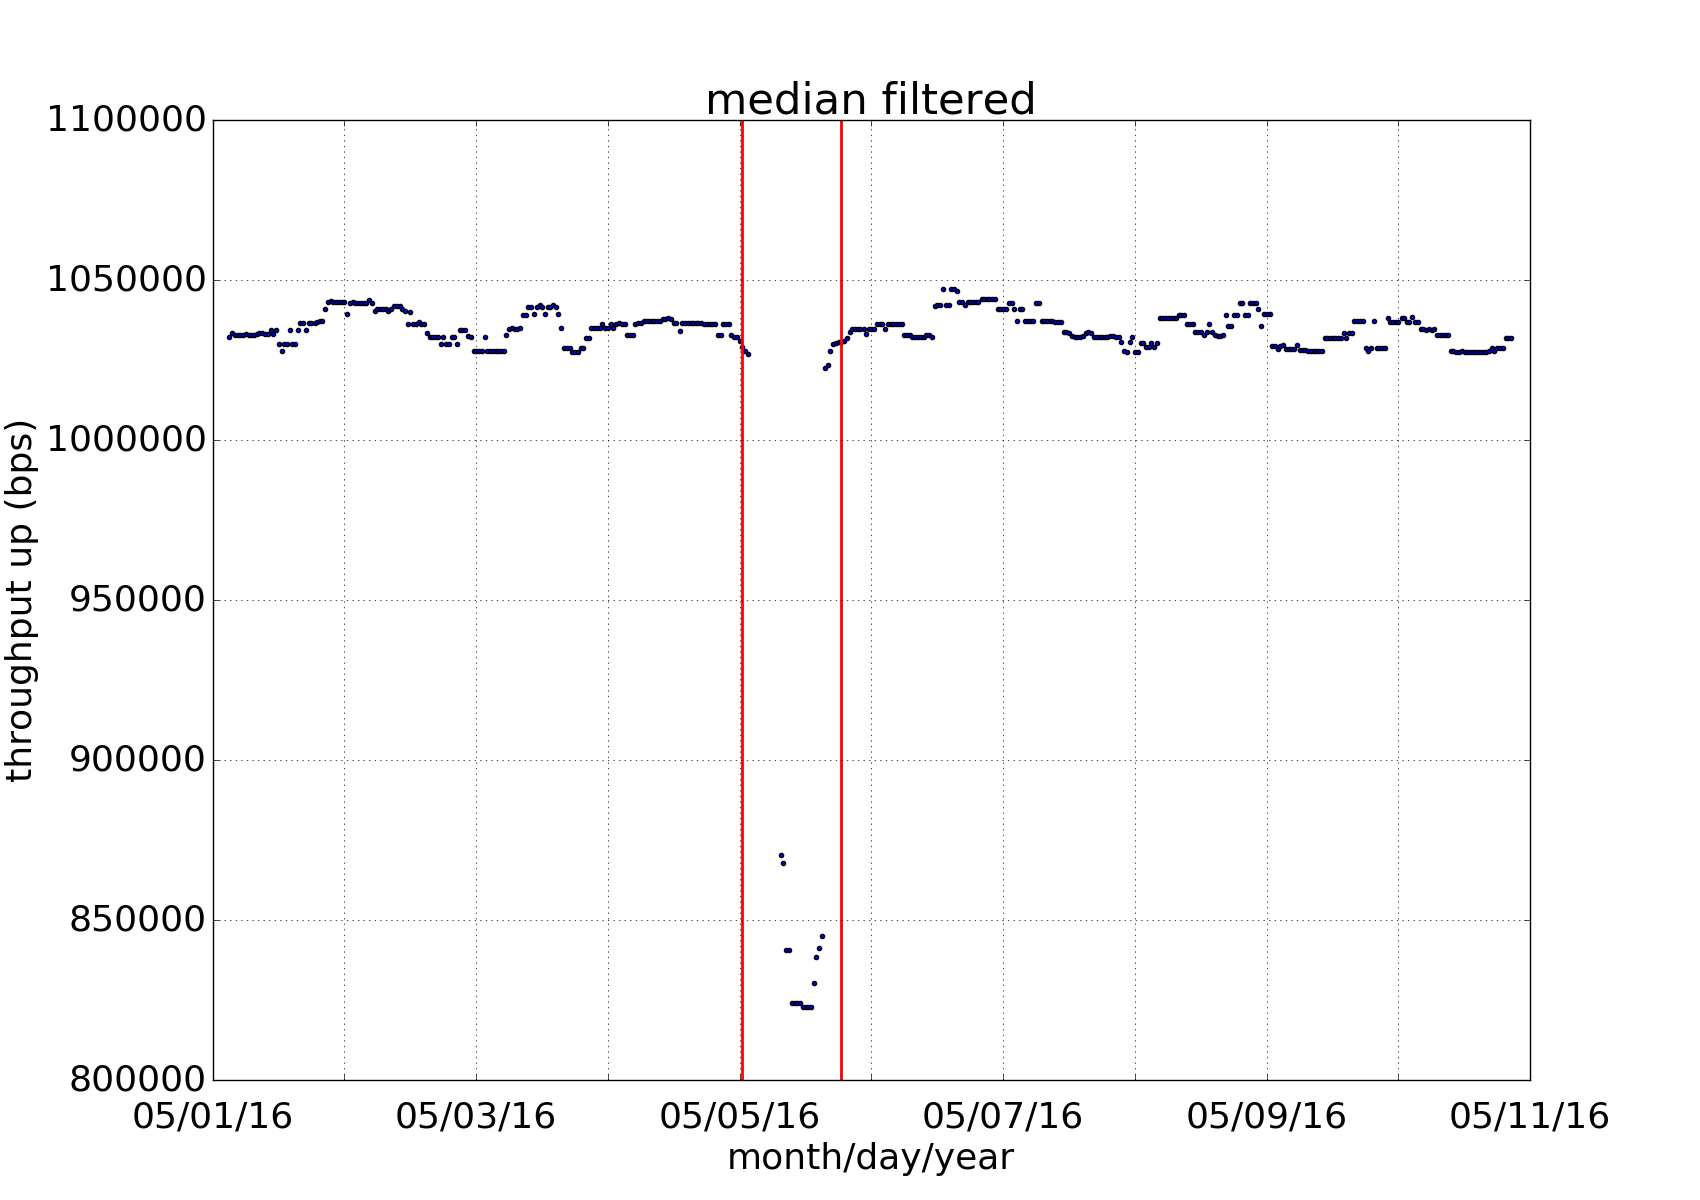
\includegraphics[width=\textwidth]{./figures/results/correct_examples/before_first_hop/serverSDRDTCLDM012_mac64:66:B3:50:06:D4_dtstart2016-05-01_dtend2016-05-11.png}
            \caption{Client 1.}
        \end{subfigure}
        \begin{subfigure}[b]{0.55\textwidth}
            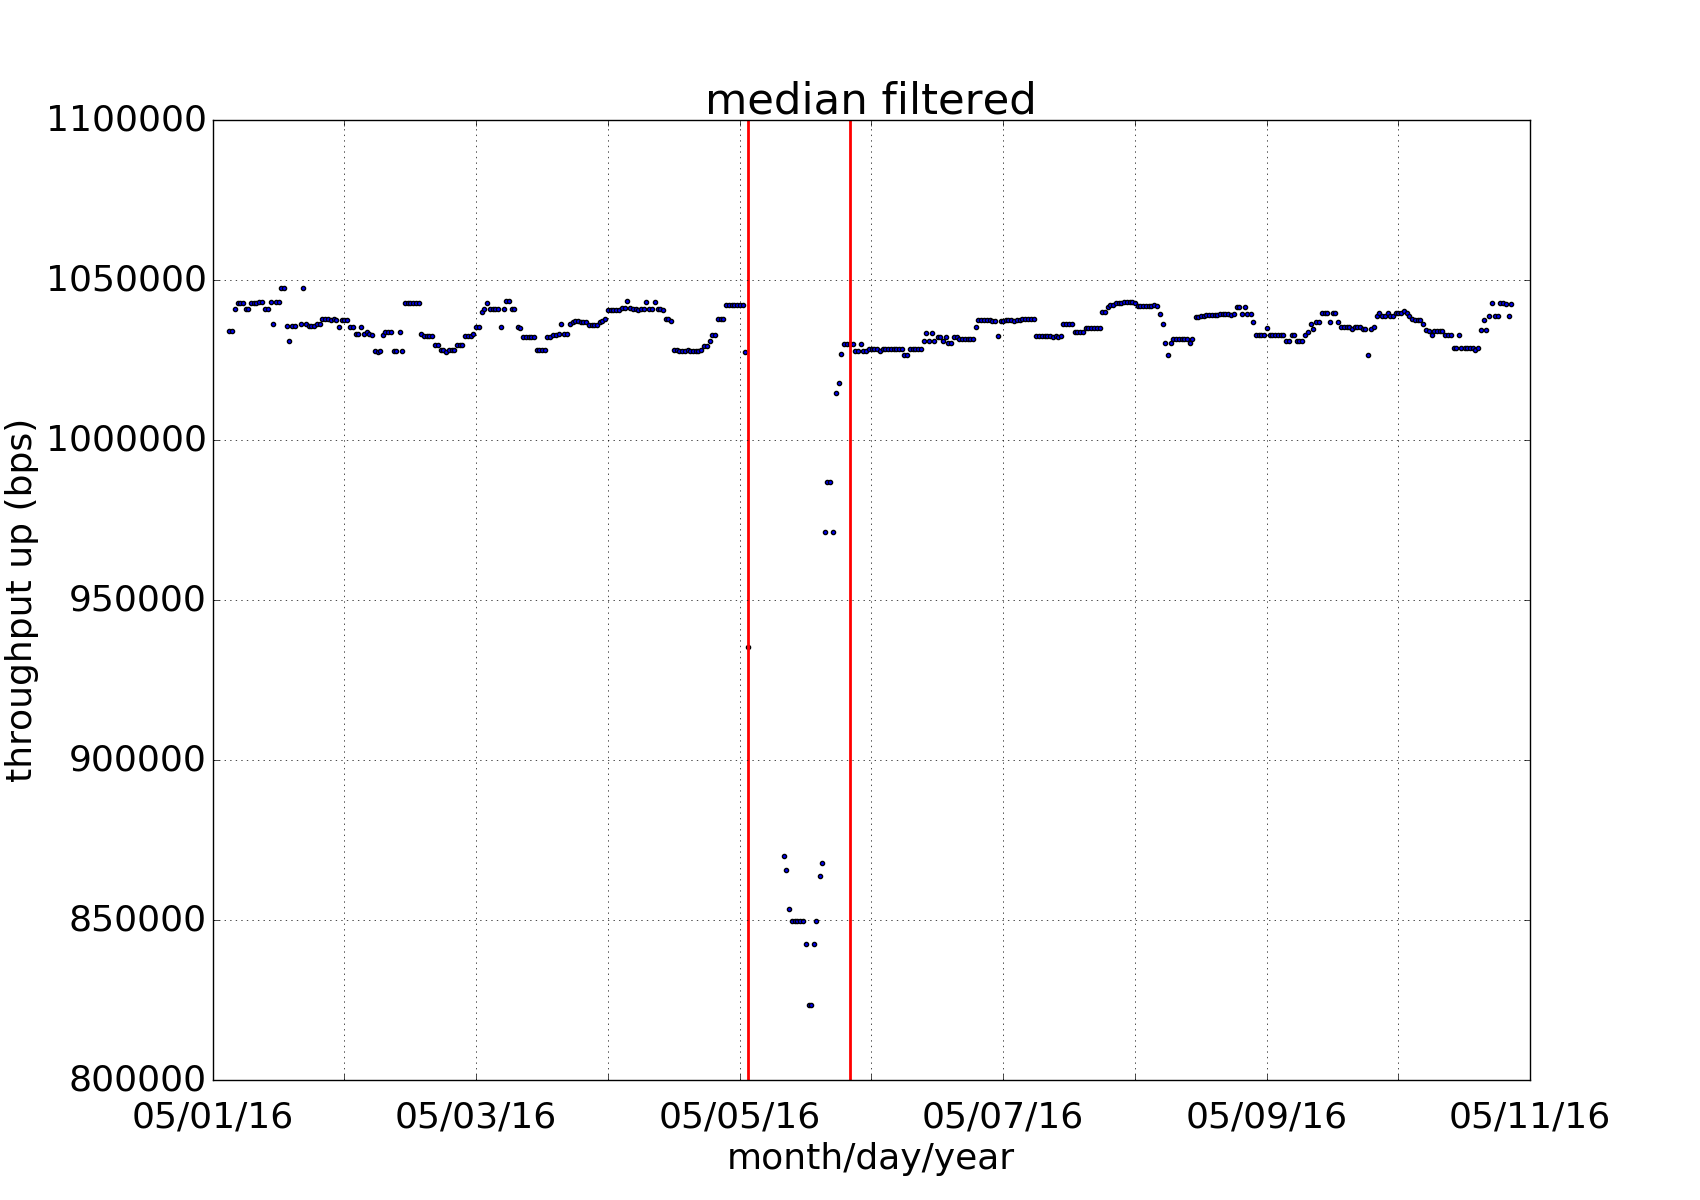
\includegraphics[width=\textwidth]{./figures/results/correct_examples/before_first_hop/serverSDRDTCLDM012_mac64:66:B3:A6:A9:70_dtstart2016-05-01_dtend2016-05-11.png}
            \caption{Client 2.}
        \end{subfigure}%
    }
    \caption{Before first hop.}
\label{fig:before_first_hop}
\end{figure}%

From the 4 clients that belong to this user-group, the system
detected the illustrated events only in these 2 customers.
Then, considering the established suppositions,
these clients must share a physical equipment before the
first hop that caused the events.

Figure~\ref{fig:zero_indegree_correlation_client} shows a client with a
specific network event, and
Figure~\ref{fig:zero_indegree_correlation_user_groups_structure} presents the
user-group structure in which this customer belong.
The vertices are defined by a tuple, in which the first field is a
label to the user-group, and the second specifies the fraction of clients
that detected the considered event.
The gray vertices represent
possible locations resulted from the analysis starting in zero indegree
user-groups.
The blue vertex indicates the correlation between these results.

\begin{figure}[H]
    \centering
    \makebox[\textwidth][c]{%
        \begin{subfigure}[b]{0.45\textwidth}
            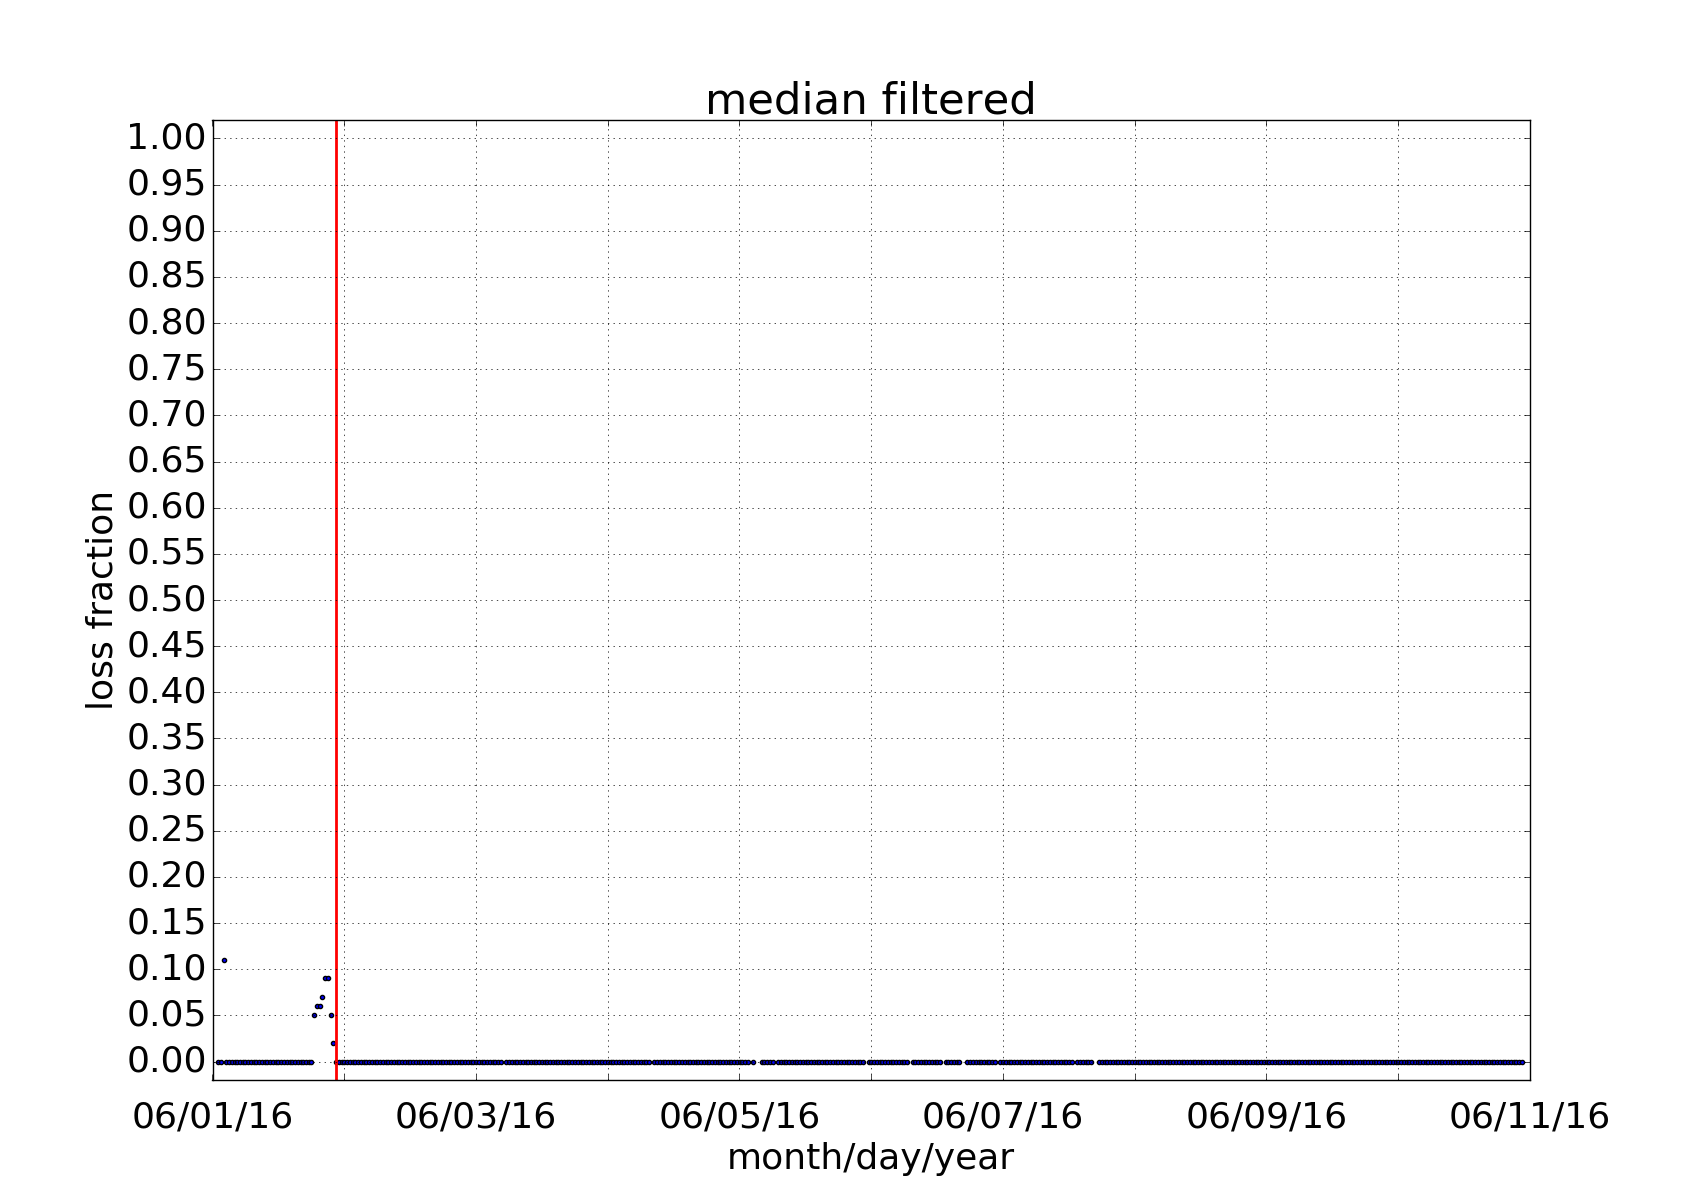
\includegraphics[width=\textwidth]{./figures/results/correct_examples/zero_indegree_correlation/serverSOCDTCPEV01_mac64:66:B3:4F:EA:E2_dtstart2016-06-01_dtend2016-06-11.png}
            \caption{Client 1.}\label{fig:zero_indegree_correlation_client}
        \end{subfigure}
        \begin{subfigure}[b]{0.7\textwidth}
            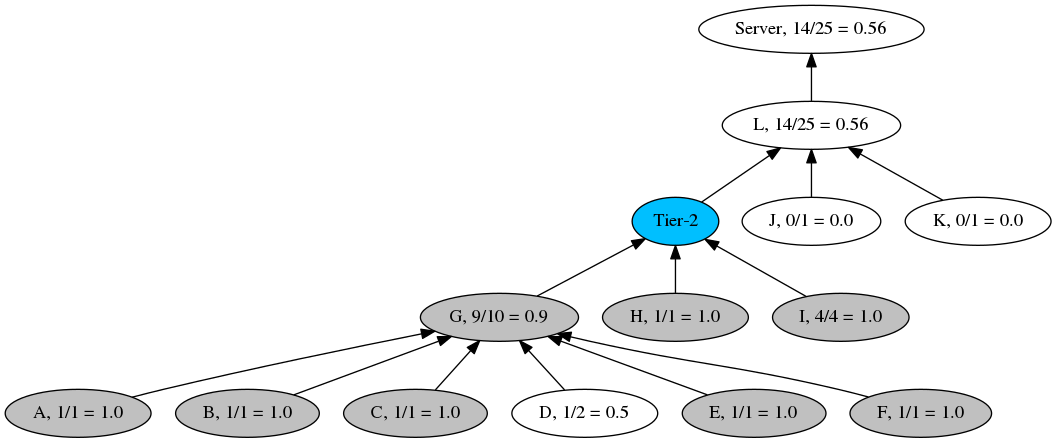
\includegraphics[width=\textwidth]{./figures/results/correct_examples/zero_indegree_correlation/dtstart2016-06-01_dtend2016-06-11_SOCDTCPEV01_traceroute_compress_embratel_graph_anonymized.png}
            \caption{User-groups structure.}\label{fig:zero_indegree_correlation_user_groups_structure}
        \end{subfigure}%
    }
    \caption{Correlation of problem locations detected by analysis that started
    in zero indegree vertices.}
\label{fig:zero_indegreee_correlation}
\end{figure}%

It was visually verified that the same change point pattern of
Figure~\ref{fig:zero_indegree_correlation_client} is present in all clients
that belong to the subtree rooted in the Tier-2 vertex.
Therefore, the system incorrectly did not detect the event in one of the D
user-group clients.
However, since several other G children detected the
event, the system's output was not compromised by this error.
Through the correlation of the zero indegree analysis,
the only match between the problem locations was the Tier-2 group.

Figure~\ref{fig:zero_indegreee_without_correlation} presents an example of a
network event that was only identified in one zero indegree user-group.

\begin{figure}[H]
    \centering
    \makebox[\textwidth][c]{%
        \begin{subfigure}[b]{0.45\textwidth}
            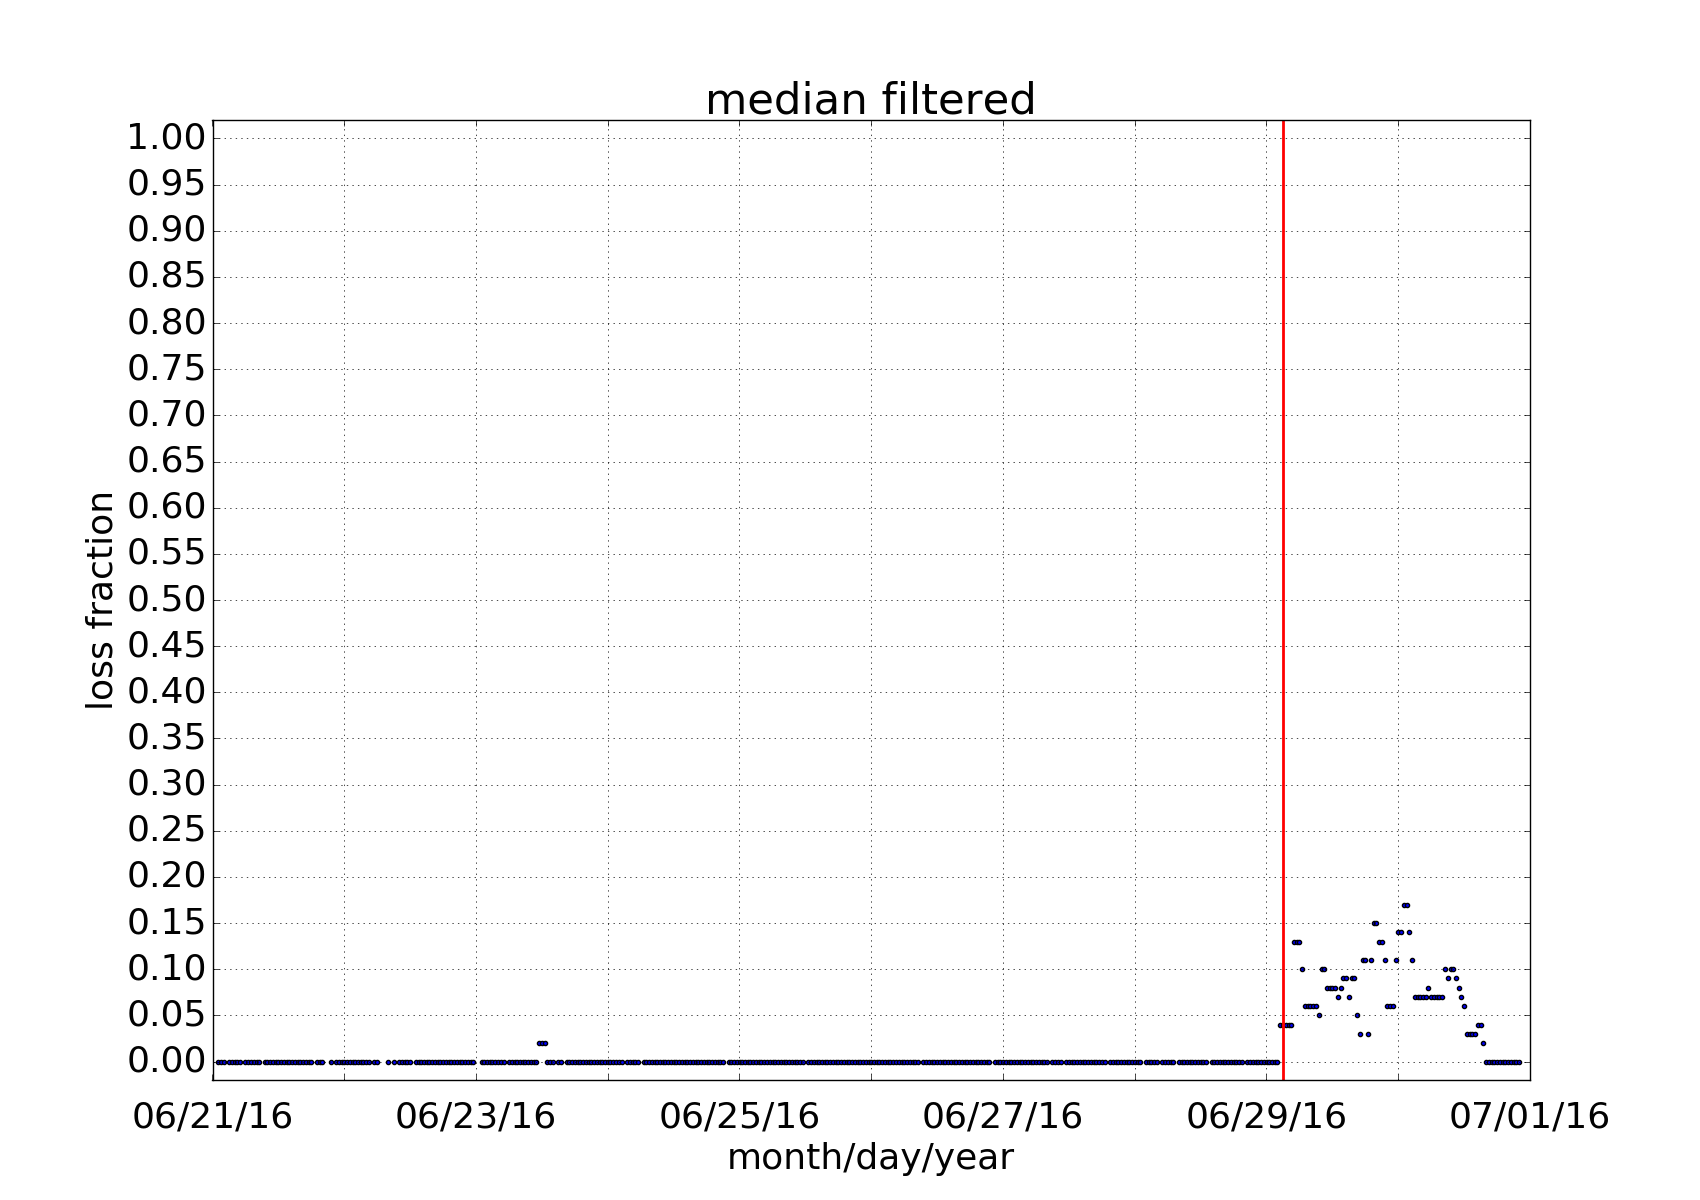
\includegraphics[width=\textwidth]{./figures/results/correct_examples/zero_indegree_single/serverGRSCBCSRV01_mac64:66:B3:50:05:56_dtstart2016-06-21_dtend2016-07-01.png}
            \caption{Client 1.}
        \end{subfigure}
        \begin{subfigure}[b]{0.7\textwidth}
            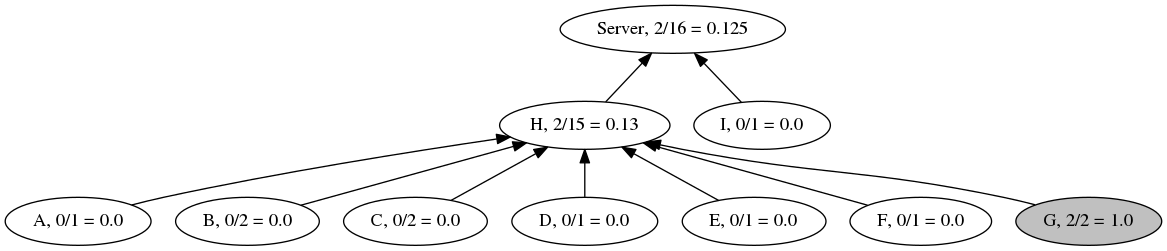
\includegraphics[width=\textwidth]{./figures/results/correct_examples/zero_indegree_single/dtstart2016-06-21_dtend2016-07-01_GRSCBCSRV01_traceroute_compress_embratel_filter_graph_anonymized.png}
            \caption{User-groups structure.}
        \end{subfigure}%
    }
    \caption{Network event in only one zero indegree user-group.}
\label{fig:zero_indegreee_without_correlation}
\end{figure}%

Table~\ref{table:number_of_events} summarizes the number of events considering
the three previous cases. The system didn't detect inconclusive events.

\begin{table}[H]
\centering
\resizebox{\textwidth}{!}{
\begin{tabular}{|c|c|c|c|c|c|c|}
\hline
\multirow{3}{*}{Metric}                & \multicolumn{6}{c|}{Events}                                                                                                                                                                                                                \\ \cline{2-7}
                                       & \multicolumn{2}{c|}{Before first hop} & \multicolumn{2}{c|}{\begin{tabular}[c]{@{}c@{}}Only one zero \\ indegree user-group\end{tabular}} & \multicolumn{2}{c|}{\begin{tabular}[c]{@{}c@{}}Multiple one degree\\ user-groups\end{tabular}} \\ \cline{2-7}
                                       & Improvement         & Failure         & Improvement                                       & Failure                                       & Improvement                                      & Failure                                     \\ \hline
RTT                                    & 688                 & 685             & 789                                               & 809                                           & 43                                               & 38                                          \\ \hline
Round trip loss fraction               & 167                 & 144             & 141                                               & 116                                           & 2                                                & 2                                           \\ \hline
Maximum achievable upstream throughput & 395                 & 358             & 331                                               & 280                                           & 4                                                & 3                                           \\ \hline
\end{tabular}
}
\caption{Number of events.}
\label{table:number_of_events}
\end{table}

\section{Possible Incorrect Outcomes}
\label{sec:possible_wrong_outcomes}

Figure~\ref{fig:time_correlation_unmatch} shows two clients that belong to
the same zero indegree user-group.

\begin{figure}[H]
    \centering
    \makebox[\textwidth][c]{%
        \begin{subfigure}[b]{0.55\textwidth}
            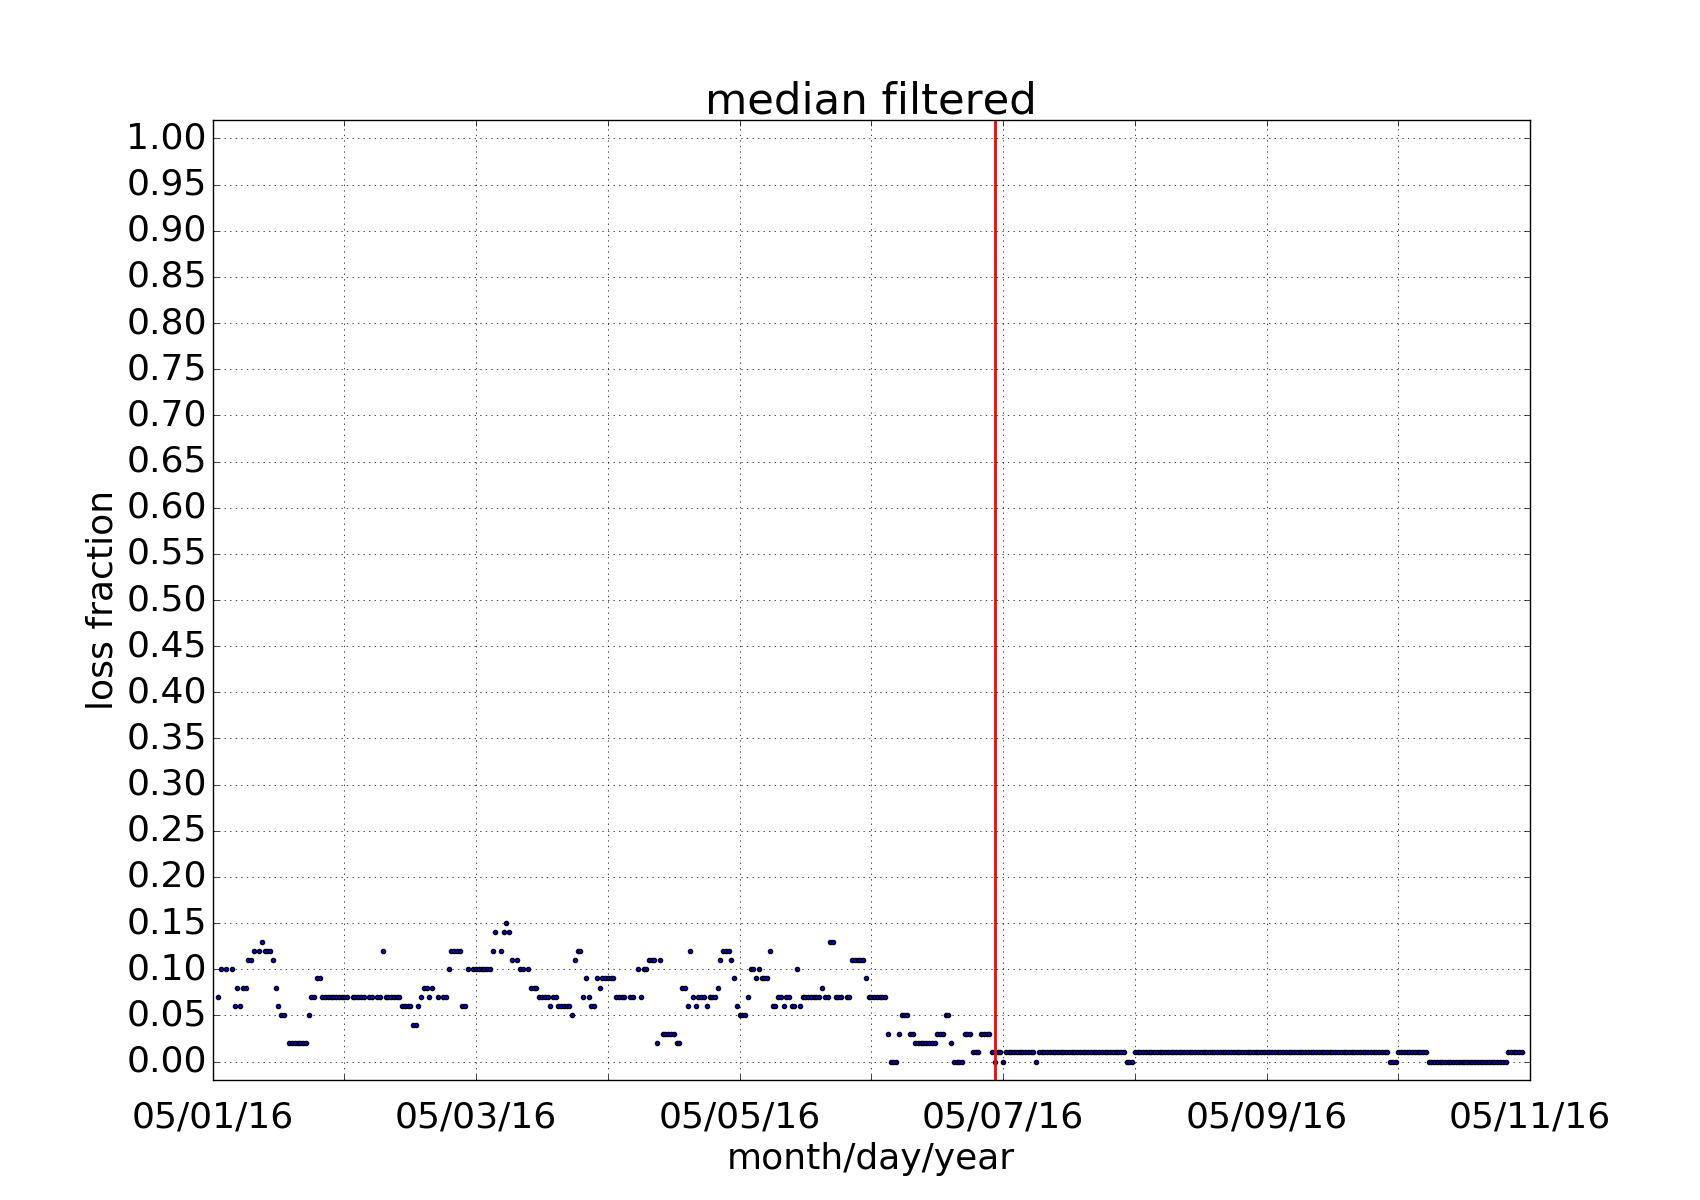
\includegraphics[width=\textwidth]{./figures/results/wrong_examples/time_correlation_example/serverSPOTVTSRV16_mac64:66:B3:A6:AB:80_dtstart2016-05-01_dtend2016-05-11.png}
            \caption{Client 1.}\label{fig:time_correlation_unmatch_client1}
        \end{subfigure}
        \begin{subfigure}[b]{0.55\textwidth}
            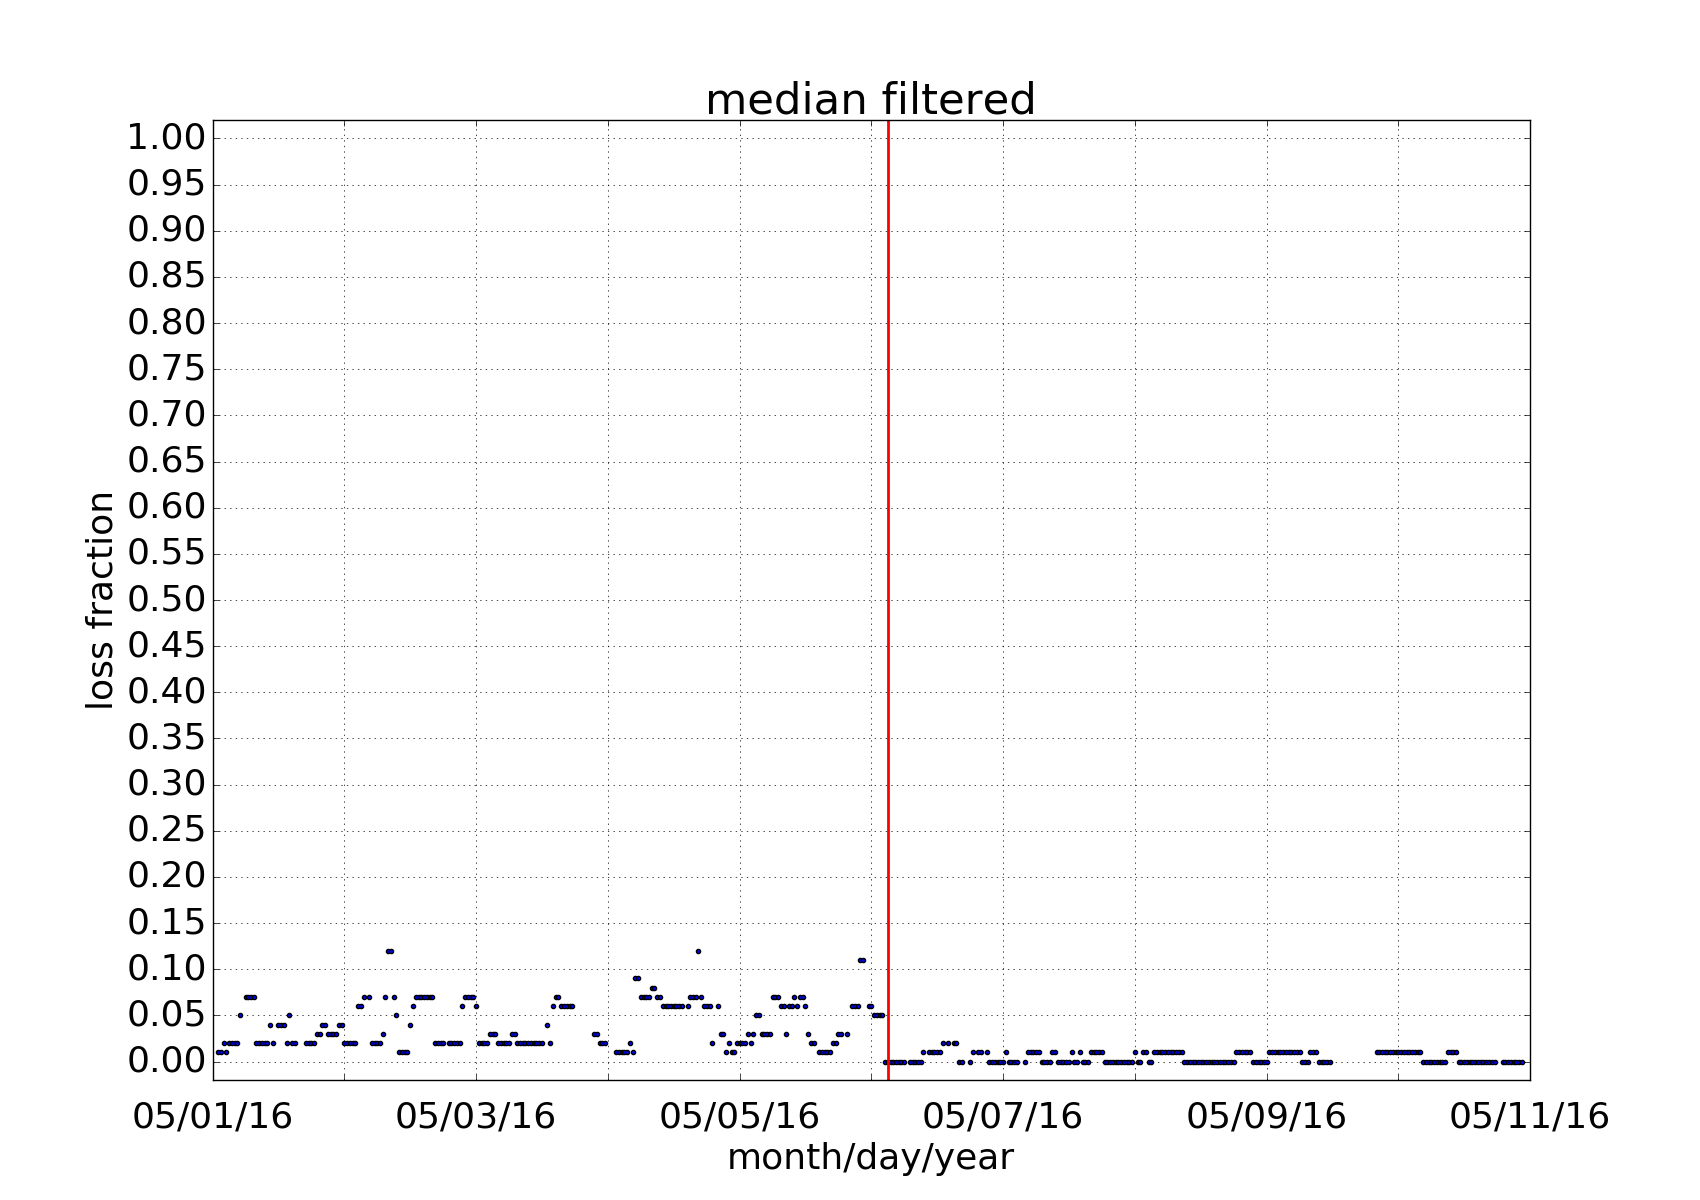
\includegraphics[width=\textwidth]{./figures/results/wrong_examples/time_correlation_example/serverSPOTVTSRV16_mac64:66:B3:A6:AC:40_dtstart2016-05-01_dtend2016-05-11.png}
            \caption{Client 2.}\label{fig:time_correlation_unmatch_client2}
        \end{subfigure}%
    }
    \caption{Time correlation unmatch.}
\label{fig:time_correlation_unmatch}
\end{figure}%

Visually, both time series have similar patterns.
However, in the left client, the change point was detected near the end of
05/07/16 day, and in the right customer, the change was identified in the
beginning of the same day.
All 17 clients of this zero indegree vertex belong to one of these two cases.
Considering the used $\delta$ value, the system recognized two different
events, nonetheless, these changes are possibly related to a single event.
This exemplifies the problem difficulty when there isn't a ground truth,
and also the importance of the algorithms and their hyperparameters selection.
Such kind of subjectivity is usual in the current dataset.

Figure~\ref{fig:untraceable_location} shows two clients that belong to the same
zero indegree vertex.

\begin{figure}[H]
    \centering
    \makebox[\textwidth][c]{%
        \begin{subfigure}[b]{0.55\textwidth}
            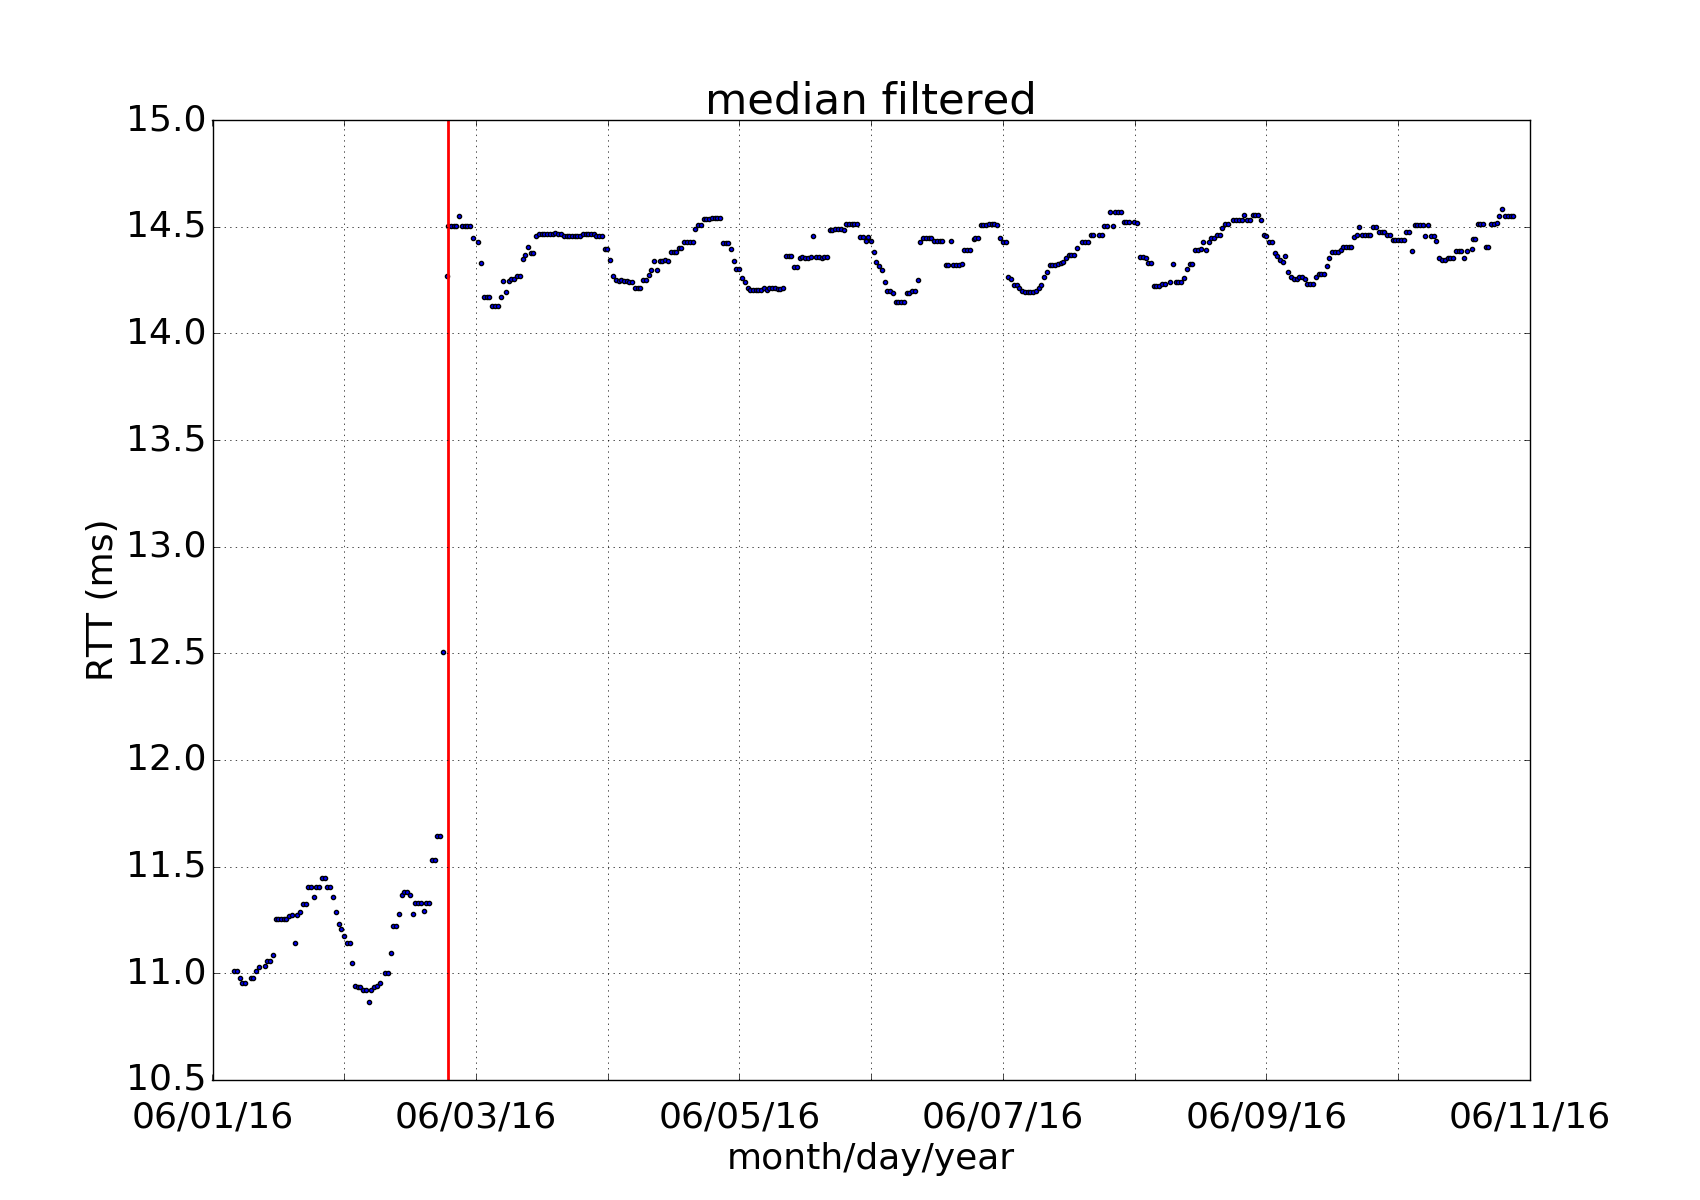
\includegraphics[width=\textwidth]{./figures/results/wrong_examples/untraceable_example/serverBHZDTCLDM062_mac64:66:B3:50:00:68_dtstart2016-06-01_dtend2016-06-11.png}
            \caption{Client 1.}\label{fig:untraceable_location_client_1}
        \end{subfigure}
        \begin{subfigure}[b]{0.55\textwidth}
            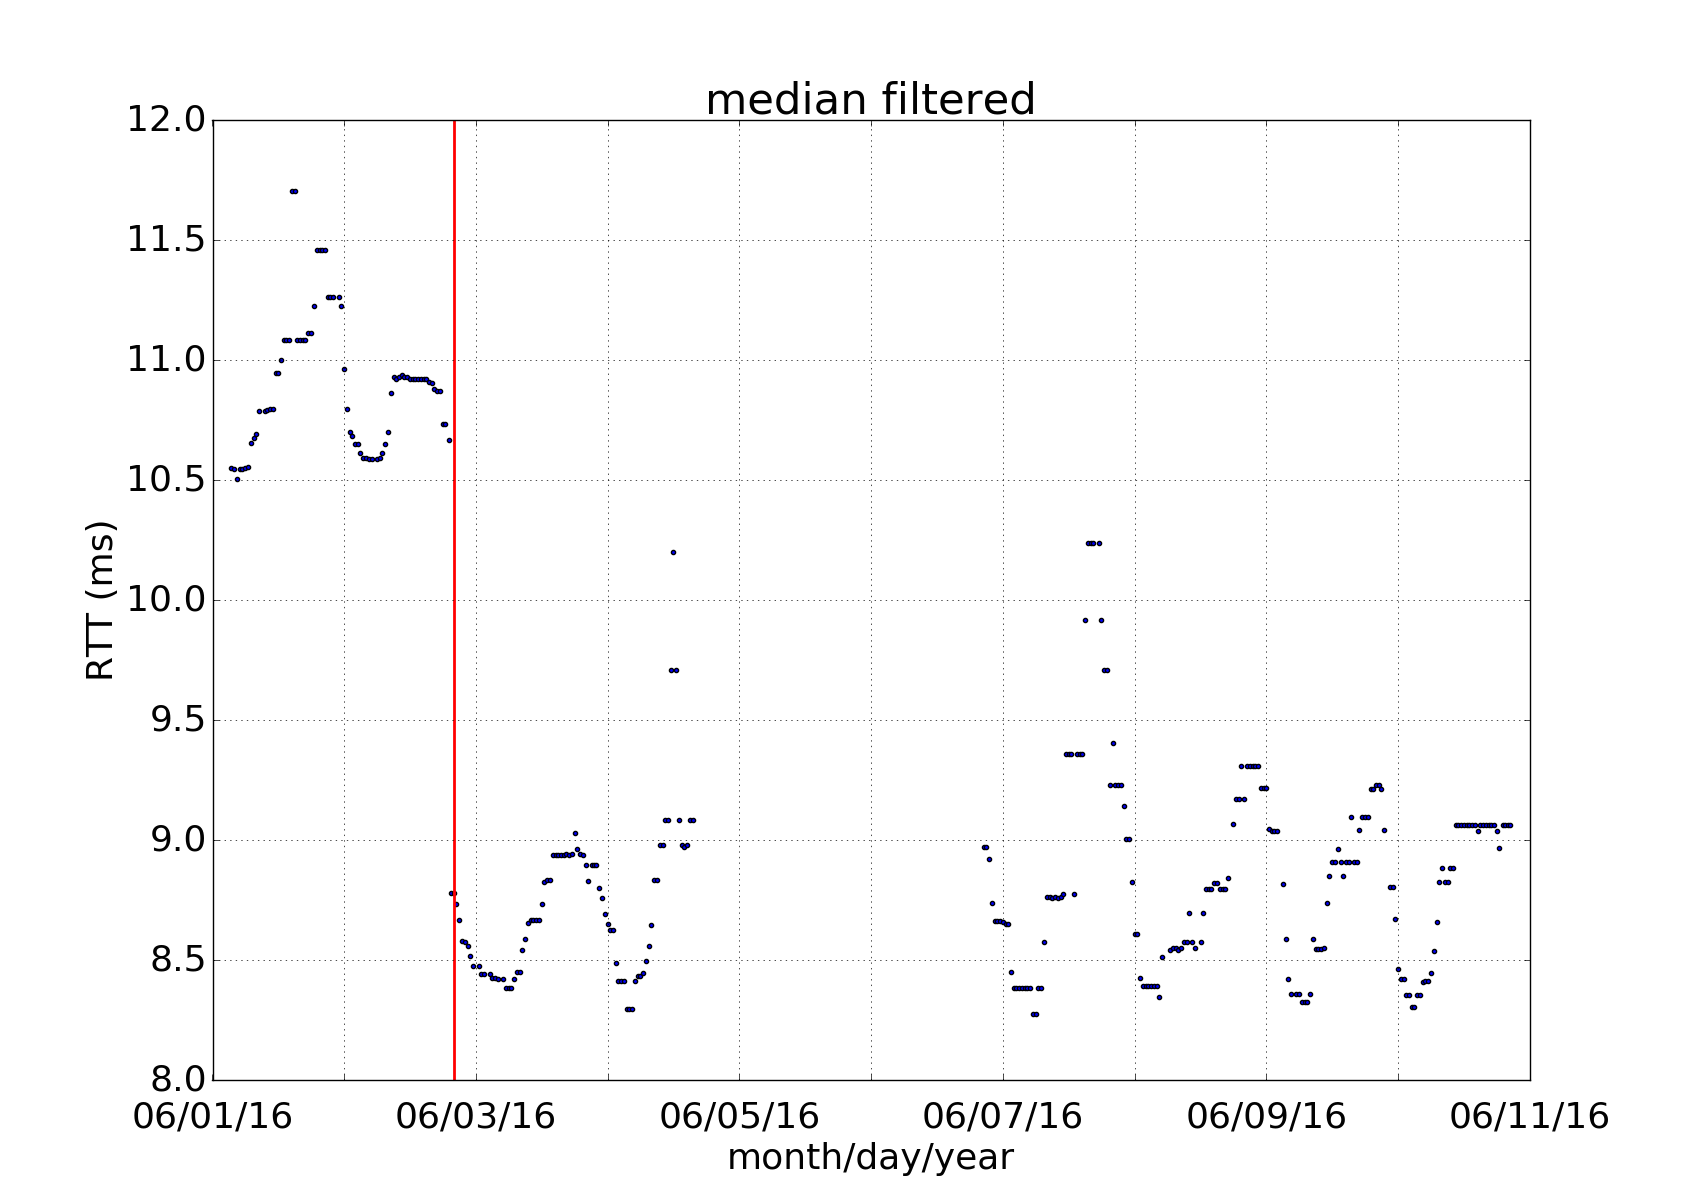
\includegraphics[width=\textwidth]{./figures/results/wrong_examples/untraceable_example/serverBHZDTCLDM062_mac64:66:B3:50:00:B6_dtstart2016-06-01_dtend2016-06-11.png}
            \caption{Client 2.}\label{fig:untraceable_location_client_2}
        \end{subfigure}%
    }
    \caption{Untraceable location.}
\label{fig:untraceable_location}
\end{figure}%

It is possible to note that both RTT time series changed their pattern
nearly at the same time, however, one case is characterized by an improvement,
while the other as a failure.
The traffic between these customers and the server
doesn't go to through the Tier-2 \gls*{isp}, therefore, according with the
suppositions, these patterns indicate simultaneous events that occurred at
different equipments before the first hop.
Nonetheless, the system detected the same RTT modifications, at the end of
06/01/16, in several other clients.
Comparing these customers, it was verified that many of them don't share
several attributes.
For instance, they executed measurements against different servers, their
upstream traffic went to completely different IP layer equipments, and they
were located at different Brazilian UFs.
This can indicate a single global network event, that simultaneously affected
different network regions. As an example, the event could be a centralized
change of DOCSIS' parameters, that is concurrently propagated to all customers.
As with local events, this work doesn't have access to this kind of
information, however, it is intriguing the fact that some of the clients
detected a failure while others perceived an improvement.
It was manually identified 3 of such cases,
and the RTT was the only impacted metric.
A significant number of RTT events were possibly wrongly classified due to this
type of event.

In general, the RTT per hop, obtained through the traceroute measurements,
can be fairly different from the analyzed RTT measures.
First, their methodologies are remarkably distinct.
Second, the RTT associated with hop $i$ can be
constantly and considerably bigger then the RTT related to a hop $j$,
where $j > i$.
This can be explained by the fact that some routers prioritizes
forwarding instead of answering ping packets.
Therefore, the analysis of this data was not included in the framework.
For instance, Figure~\ref{fig:rtt_per_hop_client_1}
presents the RTT per hop, disregarding the server hop, of the client of
Figure~\ref{fig:untraceable_location_client_1}.

\begin{figure}[H]
    \centering
    \makebox[\textwidth][c]{%
        \begin{subfigure}[b]{0.55\textwidth}
            \includegraphics[width=\textwidth]{{./figures/results/wrong_examples/untraceable_example/rtt_per_hop/64:66:B3:50:00:68/hop00_b3ea1801.virtua.com.br}.png}
            \caption{Hop 1}\label{fig:hop_1_client_1}
        \end{subfigure}
        \begin{subfigure}[b]{0.55\textwidth}
            \includegraphics[width=\textwidth]{{./figures/results/wrong_examples/untraceable_example/rtt_per_hop/64:66:B3:50:00:68/hop01_b3ea0001.virtua.com.br}.png}
            \caption{Hop 2}\label{fig:hop_2_client_1}
        \end{subfigure}
    }
    \makebox[\textwidth][c]{%
        \begin{subfigure}[b]{0.55\textwidth}
            \includegraphics[width=\textwidth]{{./figures/results/wrong_examples/untraceable_example/rtt_per_hop/64:66:B3:50:00:68/hop02_c911a615.virtua.com.br}.png}
            \caption{Hop 3}\label{fig:hop_3_client_1}
        \end{subfigure}
        \begin{subfigure}[b]{0.55\textwidth}
            \includegraphics[width=\textwidth]{{./figures/results/wrong_examples/untraceable_example/rtt_per_hop/64:66:B3:50:00:68/hop03_c91180fe.virtua.com.br}.png}
            \caption{Hop 4}\label{fig:hop_4_client_1}
        \end{subfigure}
    }
    \caption{RTT per hop of client of
    Figure~\ref{fig:untraceable_location_client_1}.}
\label{fig:rtt_per_hop_client_1}
\end{figure}%

It is not possible to visually identify the same change pattern of
Figure~\ref{fig:untraceable_location_client_1} in the hops analysis.
Figure~\ref{fig:rtt_per_hop_client_2} is analogous, however, related to client
of Figure~\ref{fig:untraceable_location_client_2}.

\begin{figure}[H]
    \centering
    \makebox[\textwidth][c]{%
        \begin{subfigure}[b]{0.55\textwidth}
            \includegraphics[width=\textwidth]{{./figures/results/wrong_examples/untraceable_example/rtt_per_hop/64:66:B3:50:00:B6/hop00_b3ea1801.virtua.com.br}.png}
            \caption{Hop 1}\label{fig:hop_1_client_2}
        \end{subfigure}
        \begin{subfigure}[b]{0.55\textwidth}
            \includegraphics[width=\textwidth]{{./figures/results/wrong_examples/untraceable_example/rtt_per_hop/64:66:B3:50:00:B6/hop01_b3ea0001.virtua.com.br}.png}
            \caption{Hop 2}\label{fig:hop_2_client_2}
        \end{subfigure}
    }
    \makebox[\textwidth][c]{%
        \begin{subfigure}[b]{0.55\textwidth}
            \includegraphics[width=\textwidth]{{./figures/results/wrong_examples/untraceable_example/rtt_per_hop/64:66:B3:50:00:B6/hop02_c911a615.virtua.com.br}.png}
            \caption{Hop 3}\label{fig:hop_3_client_2}
        \end{subfigure}
        \begin{subfigure}[b]{0.55\textwidth}
            \includegraphics[width=\textwidth]{{./figures/results/wrong_examples/untraceable_example/rtt_per_hop/64:66:B3:50:00:B6/hop03_c91180fe.virtua.com.br}.png}
            \caption{Hop 4}\label{fig:hop_4_client_2}
        \end{subfigure}
    }
    \caption{RTT per hop of client of
    Figure~\ref{fig:untraceable_location_client_2}.}
\label{fig:rtt_per_hop_client_2}
\end{figure}%

In this case, it can be noticed that the RTT is bigger in the beginning of the
first hop time series.
This same pattern was detected in the RTT between the client and the server.

\section{Final Remarks}

Various events related to the maximum achievable upstream
throughput, consist of a substantial mean increase perceived by a single client,
as is exemplified in Figure~\ref{fig:throughput_up_increase}.
Possibly this type of event indicates a change in the customer's contracted
bandwidth.

\begin{figure}[H]
    \centering
    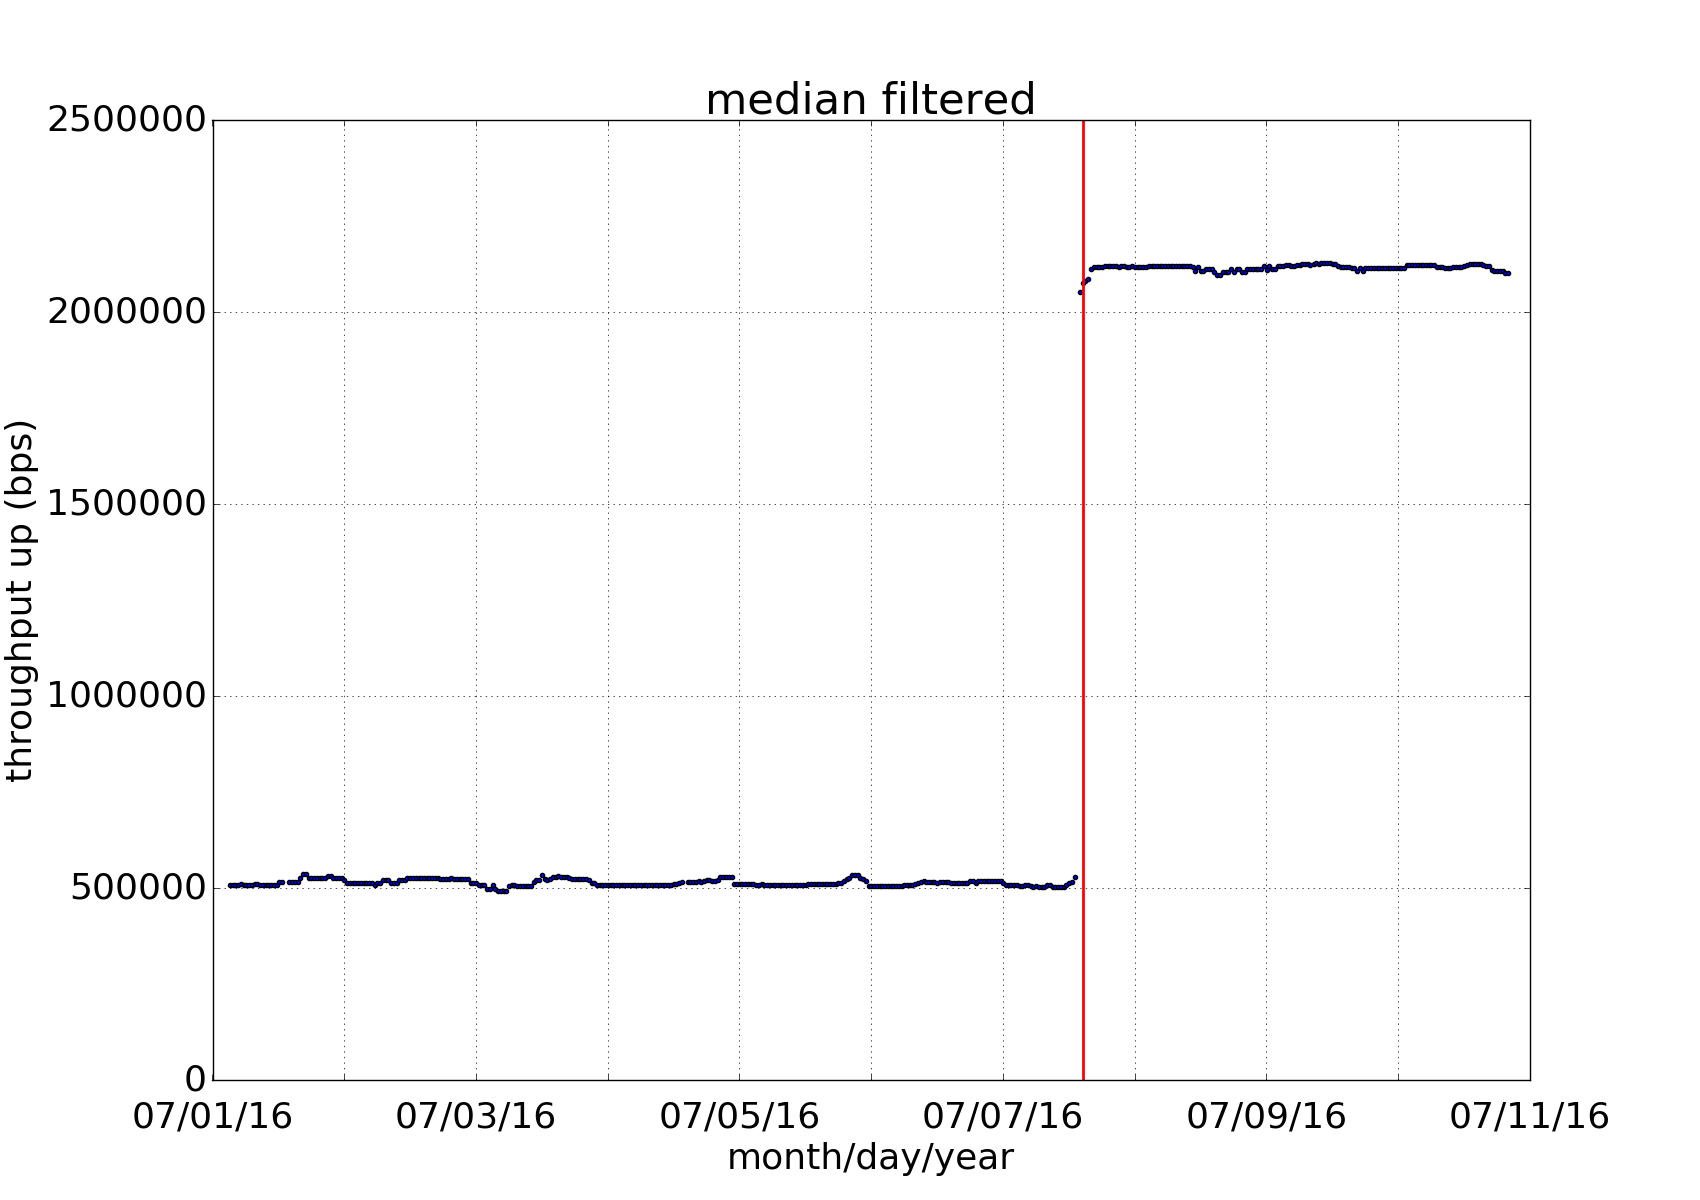
\includegraphics[width=0.7\linewidth]{./figures/results/final_remarks/change_contracted_bandwidth/serverGOIDTCSRV07_macF8:1A:67:2E:E4:9A_dtstart2016-07-01_dtend2016-07-11.png}
    \caption{Possible contract bandwidth change.}
\label{fig:throughput_up_increase}
\end{figure}%

Several problem locations are supported by a change point detected in a single
client.
Figure~\ref{fig:clients_sparsity} exhibits an example.

\begin{figure}[H]
    \centering
    \makebox[\textwidth][c]{%
        \begin{subfigure}[b]{0.45\textwidth}
            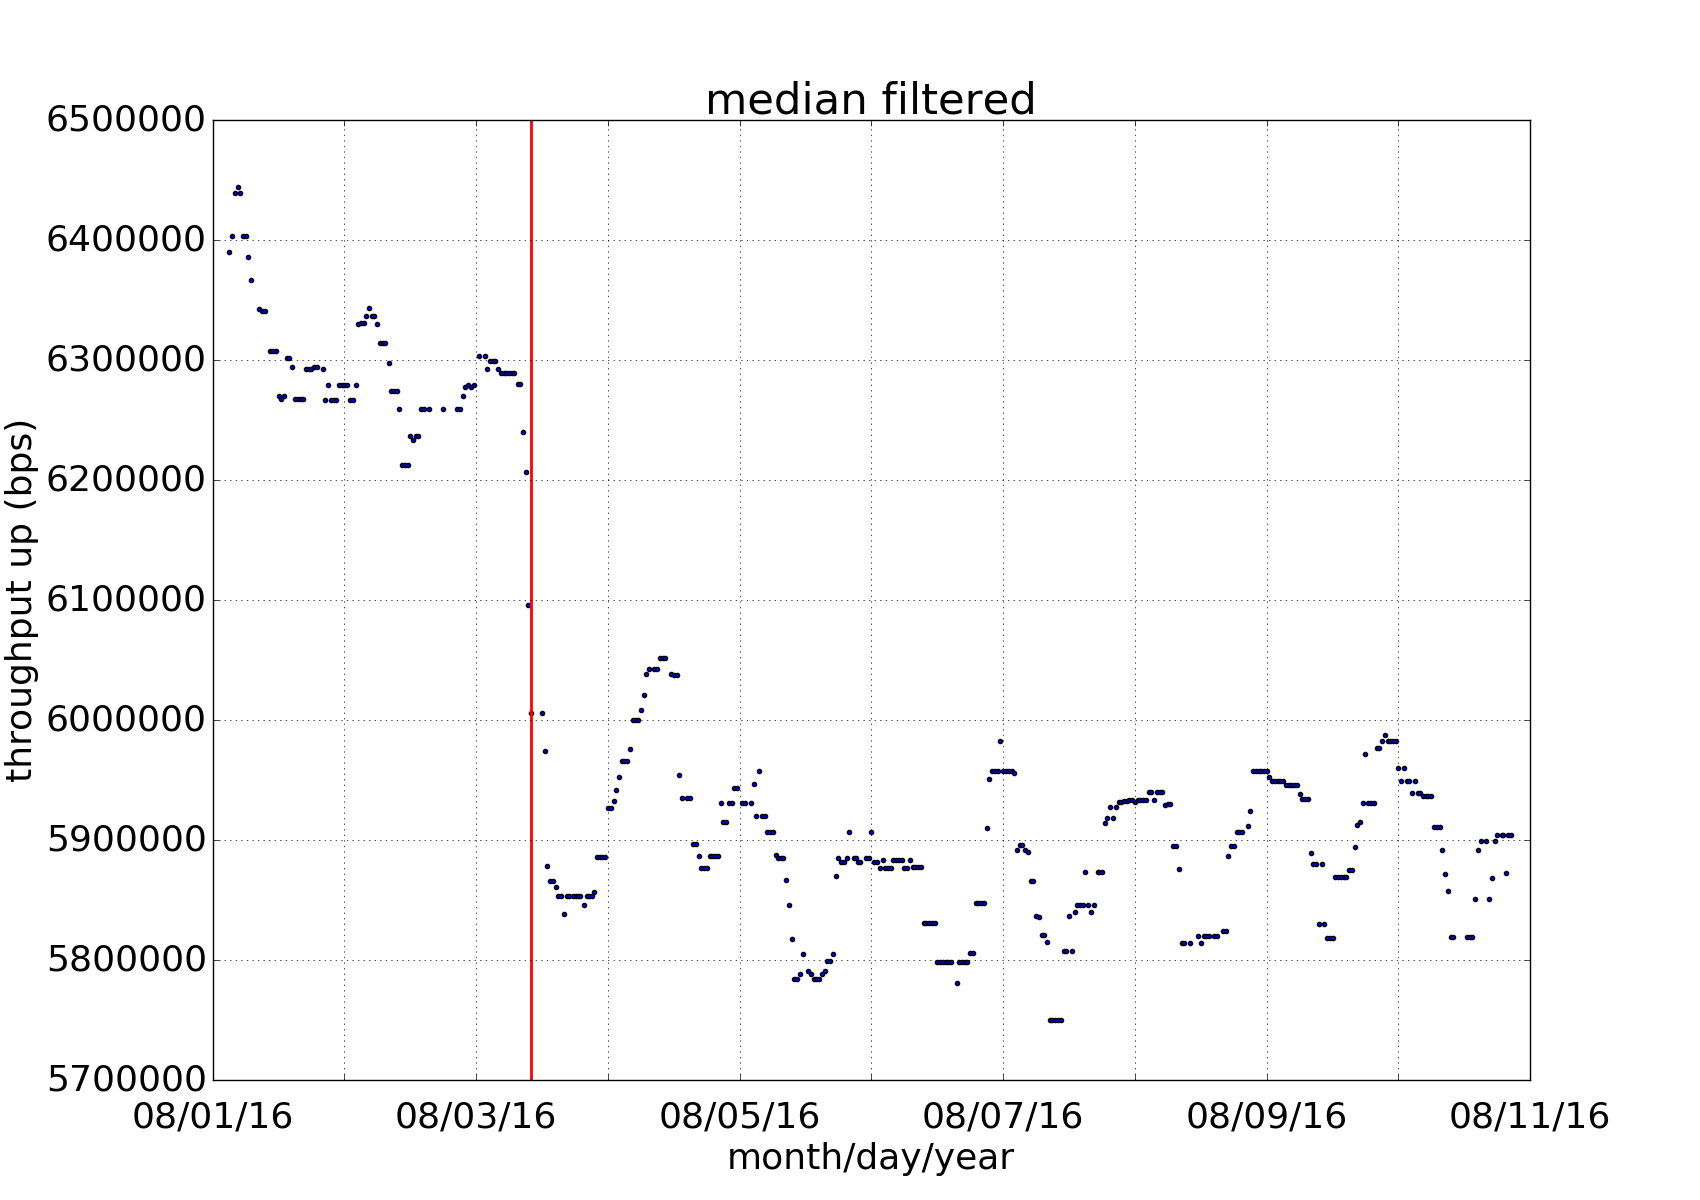
\includegraphics[width=\textwidth]{./figures/results/final_remarks/client_sparsity/serverRJODTCLDM031_mac64:66:B3:4F:E9:24_dtstart2016-08-01_dtend2016-08-11.png}
            \caption{Client 1.}
        \end{subfigure}
        \begin{subfigure}[b]{0.7\textwidth}
            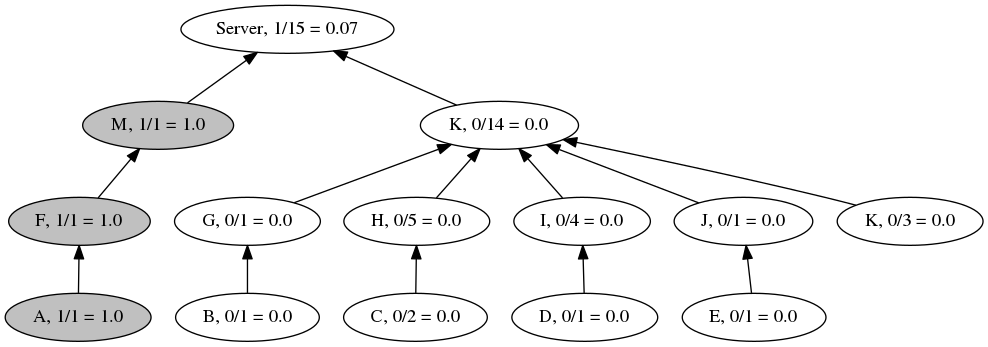
\includegraphics[width=\textwidth]{./figures/results/final_remarks/client_sparsity/dtstart2016-08-01_dtend2016-08-11_RJODTCLDM031_traceroute_compress_embratel_filter_subgraph_anonymized.png}
            \caption{User-groups structure.}
        \end{subfigure}%
    }
    \caption{Clients sparsity.}
\label{fig:clients_sparsity}
\end{figure}%

It is not possible to exactly locate the event,
since the three gray vertices are composed by the same end-user.
This can be avoided with an appropriate selection of the tracked customers.
For instance,
Figure~\ref{fig:number_of_clients_per_zero_indegree_vertex} presents
the number of clients per zero indegree vertex histogram.
More than 70\% of the zero indegree vertices have only one client.

\begin{figure}[H]
    \centering
    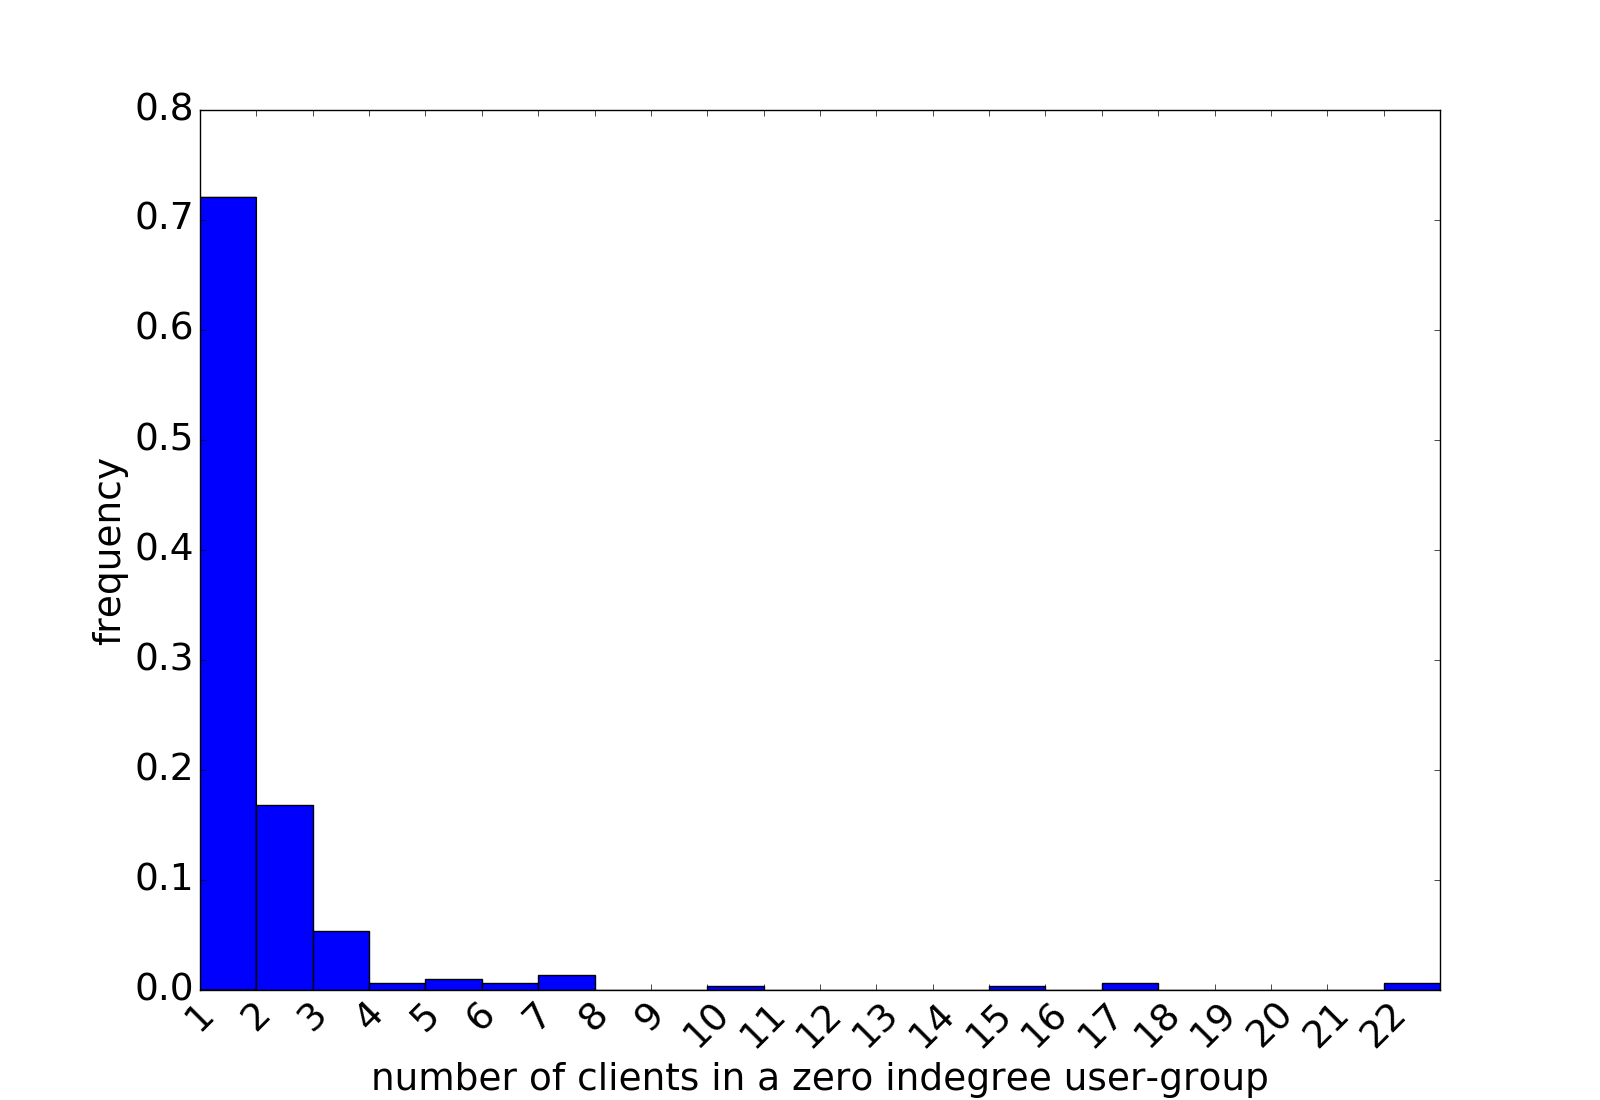
\includegraphics[width=0.7\linewidth]{./figures/results/final_remarks/cnt_clients_zero_indegree_vertex_distribution.png}
    \caption{Number of clients per zero indegree user-group histogram.}
\label{fig:number_of_clients_per_zero_indegree_vertex}
\end{figure}%
